\chapter{Reconstruction} % 

The precise measurement of particles produced in the high energy collisions at the LHC 
is necessary to effectively execute the CMS physics programme. This requires effective
reconstruction and identification of physics objects in a challenging environment containing
large numbers of different particles with a range of energies. The \alphat analysis 
relies directly on reconstruction of jets and \met for the signal region and on the 
reconstruction of leptons and photons to reject backgrounds and define control regions.
This requires the use of information from all detector subsystems and state-of-the-art
techniques for reconstruction, selection and calibration of physics objects to ensure 
an optimal performance. 

\section{Detector reconstruction}

The first stage in reconstructing the physics objects is to produce the necessary
input information from the detector subsytems. This takes the form of both the tracks, 
trajectories, of charged particles as well as the energy measurements from
calorimeter depositions. Specialist algorithms which suppress backgrounds, 
mitigate the effects of pileup and provide high resolution energy,
position and/or temporal measurements are used to optimise the precision of the 
measured quantities over a wide range of particle energies and momenta.

\subsection{Track reconstruction}

Charged particle tracks are reconstructed from the hits, considering the efficiency and resolution, 
using the iterative Combinatorial Track Finder (CTF) algorithm. The track reconstruction can be decomposed 
into four logical steps outlined below.

\begin{itemize}
\item Seeds are generated using either triplets of tracker hits or pairs of hits with an additional constraint 
from the beamspot or a pixel vertex. This gives an initial estimate of the trajectory with uncertainty \cite{tracker_early}.
\item Each seed is propagated outward through the tracker layers considering the current uncertainty in the trajectory.
In propagating, a uniform magnetic field as well as no energy loss or multiple Coulomb scattering effects are assumed.
The track parameters are then updated with the best matching hit on each layer (if any) according to the Kalman filter formalism \cite{tracker_vertex}.
The search continues until either the boundary of the tracker is reached or no more compatible hits are found. If a minimum number
of valid hits are observed an inwards search is initiated for additional hits\cite{tracker_early}.
\item It is possible for a single charged particle track to be reconstructed more than once, starting either from different seeds or if
one seed develops into multiple track candidates. If the fraction of shared hits between two track candidates is greater
than 19\% (determined empirically) the track with fewer hits is discarded. If the number of hits is equivalent the track with
 the largest $\chi^2$ is discarded\cite{tracker_vertex}.
\item After the track candidates are built and cleaned the hits in each candidate are refitted using a Kalman filter and smoother. This 
avoids possible bias from the seeding stage \cite{tracker_vertex}.
\end{itemize}

The CTF performs six iterations to determine the tracks. Between each iteration any hits that are assigned to tracks in the
previous iteration are removed from the collection. The final track collection is then filtered to remove fake tracks using 
information on the number of hits, the $\chi^2$ and the compatibility of the track originating from a pixel vertex. The momentum 
resolution achieved is 0.7 (5)\% at 1 (1000) \GeV in the central region\cite{tracker_early}. Using a dataset of pions and muons from an early run 
at the LHC the tracking efficiency was measured as 98\% for tracks with $p_T > 500\MeV$ and $>99\%$ for tracks with $p_T > 2\GeV$\cite{tracker_eff}.

\subsection{Vertex Reconstruction}

As described in Sec.~\ref{lhc_intro}, the LHC produced an average of 25 simultaneous collisions per bunch crossing
during Run 2. It is essential to identify the Primary Vertex (PV) and the particles originating from it to allow 
particles from additional collisions to be rejected and to identify features such as displaced vertices. The tracks
are initially clustered using a deterministic annealing (DA) algorithm based on the points of closest approach of the 
tracks to the beamspot \cite{tracker_vertex}. The candidate vertices containing at least two tracks are then
fitted using an adaptive vertex fitter (AVF) to compute the best estimates of vertex parameters \cite{tracker_avf}. 
Each track in the vertex is assigned a weight between 0 and 1 corresponding to the likelihood that that track
belongs to the vertex. The tracks with weight near 1 are most consistent with the reconstructed vertex while
those that are least consistent have small weights. The number of degrees in the fit, defined as 

\begin{equation}
n_{dof} = -3 + 2 \sum_{i=1}^{\#tracks} wi,
\end{equation}

is an important parameter for distinguishing real proton-proton interactions from misclustered vertices as it is strongly corrected with
the number of tracks compatible with arising from the interaction region \cite{tracker_vertex}. The vertex
position and resolution determined using the AVF have been 
measured in early LHC data and compared with simulation as shown in Fig~\ref{fig:pvEffRes}.

\begin{figure}[hbt]
  \begin{center} 
   \subfigure[\label{fig:pvEff}]{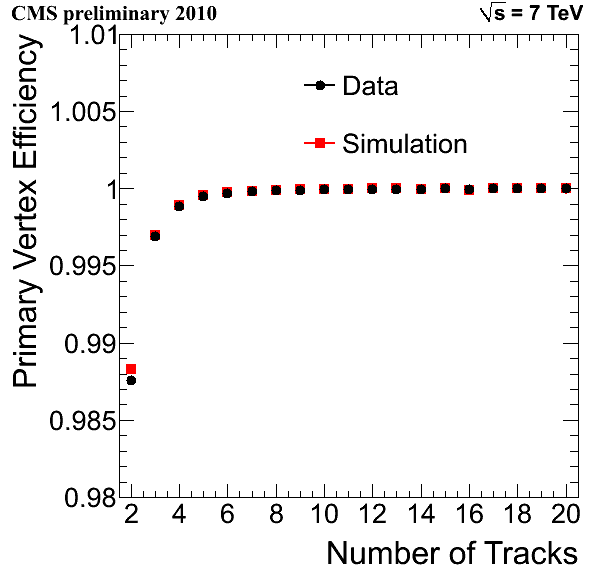
\includegraphics[width=0.5\textwidth]{Figures/detector/pvEff}}~
   \subfigure[\label{fig:pvRes}]{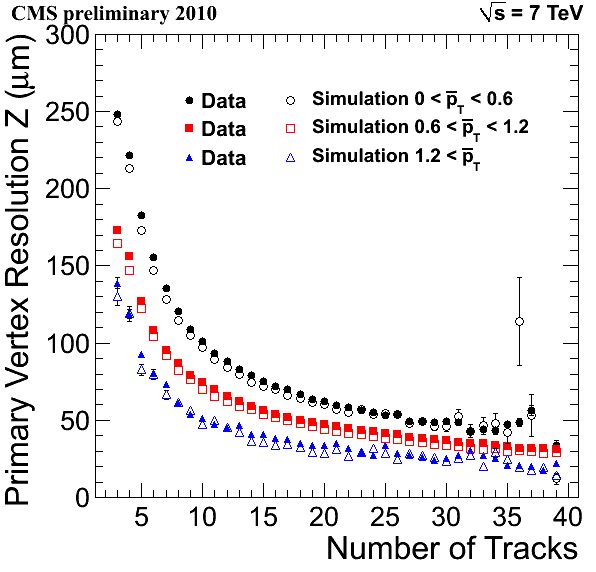
\includegraphics[width=0.5\textwidth]{Figures/detector/pvRes}}
   \caption{(a) Primary Vertex efficiency as a function of the number of associated tracks. (b) Primary Vertex 
   resolution in the z coordinate as a function of the number of associated tracks for three track $p_T$ scenarios \cite{tracker_seven}
   \label{fig:pvEffRes} }
  \end{center}
\end{figure}

The vertices are ordered according to the sum of the $p_T^2$ of the tracks associated to each vertex with the 
vertex with the highest $p_T^2$ taken as the primary vertex (PV). The position of the primary vertex can
be used for object identification and control of pile-up. Many CMS analyses, including the one in this 
thesis, make requirements that a good vertex is reconstructed from the tracks satisfying:

\begin{itemize}
\item A minimum number of degrees of freedom: $n_{dof} > 4$.
\item The collision to occur with $|z| < 24cm$ such that the primary vertex is near the interaction point in the longitudinal direction.
\item The collision to occur within a radial distance of $|d_{xy}| < 24cm$ from the beamline.
\end{itemize}

\subsection{Calorimeter reconstruction}

The calorimeters must reconstruct the energies of incident particles from the energy deposits made in the 
various subsystems. These deposits must be clustered and the measurement calibrated to provide 
details of the energy, position and timing of the incident particle. These can be used to complement 
the information from the tracker and provides necessary redundancy in the case of track
misreconstruction. For neutral particles the calorimeter subsystems provide the only measurement of
the particle properties. In Section ??, details of how the complementary information from the calorimeter
with the tracking and muon subsystems is used to identify particles and reconstruct the event.

The ECAL crystals are calibrated with both absolute and relative calibrations. Nine of 36 EB superclusters
and 500 EE crystals are calibrated using high energy electron beams to achieve a resolution of 0.5\% (1\%) for the EB (EE) components. 
The remainder undergo relative intercalibration to achieve a resolution of 1.4\%-1.8\% ($\sim5\%$) for the EB (EE) components. 
During running the response of the crystals changes due to radation induced crystal-lattice defects which absorb the scintillation light. 
The crystal transparency is monitored to allow the impact on energy measurements to be assessed and corrected \cite{ecal_calib}. 
The HCAL components undergo a similar calibrartion to the ECAL crystals. Firstly a subset of the components are calibrated with
a 50GeV pion beam and this is then extended to the remainder of the subsystem using a Co source \cite{hcal_beam}. Additional corrections are derived during 
LHC running \cite{hcal_calib}.

The reconstruction of the energy at the HCAL and ECAL relies on recording the amplified light pulses from the photodiodes over a 25ns time
sample. When operating with 25ns bunch spacing particle energies from previous or following bunch crossings can be integrated
into this sample, biasing the energy measurement. This effect is correcting by using a dedicated reconstruction that removes
the contributions from such Out Of Time Pileup (OOTPU)~\cite{hcal_timing,ecal_timing}. The 25ns sample is fitted including three pulse shape templates with
variable amplitude and arrival times with the central pulse corresponding to the triggered event. The timing distribution for
the ECAL hits above 1GeV, which is derived indepedantly from the energy measurement, is shown in Figure~\ref{fig:timing_barrel_linear} showing that
contributions from OOTPU are rejected.

\begin{figure}
\centering
    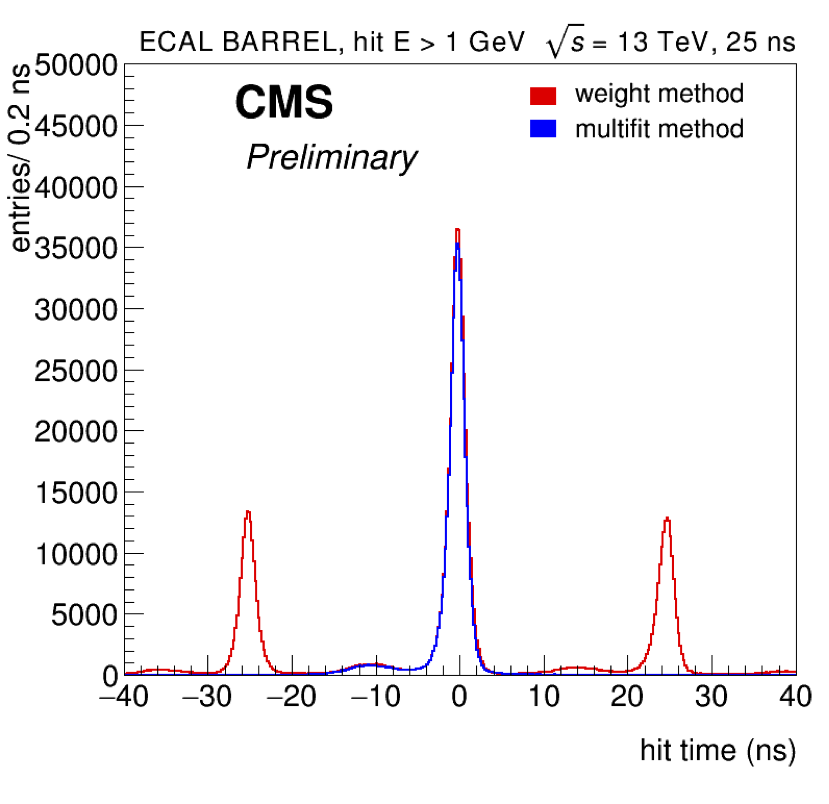
\includegraphics[width=0.8\textwidth]{./Figures/reconstruction/timing_barrel_linear.png}
  \caption{Timing distribution of the hits in the ECAL barrel with a reconstructed energy above 1 GeV~\cite{ecal_timing}.}
  \label{fig:timing_barrel_linear}
\end{figure}
